


\subsection{Humidty sensor push information}

\hrule
\hfill
\vspace{0.5cm}
\label{operation:Humidty sensor push information}

The Humidity Sensor pushes the information to the sensor table.
\begin{description}
\item \textbf{Parameters:} 
\item \textbf{Precondition:} The system is bootedup with the respected
configurations.
\item \textbf{Post-condition:} Updated sensor value in sensor table.
 
\item \textbf{Triggering:}
\begin{enumerate}
\item \textbf{Humidity sensor} send digital signal to the system.
\item System updates the value of the given sensor in the sensor table.
\begin{figure}[H]
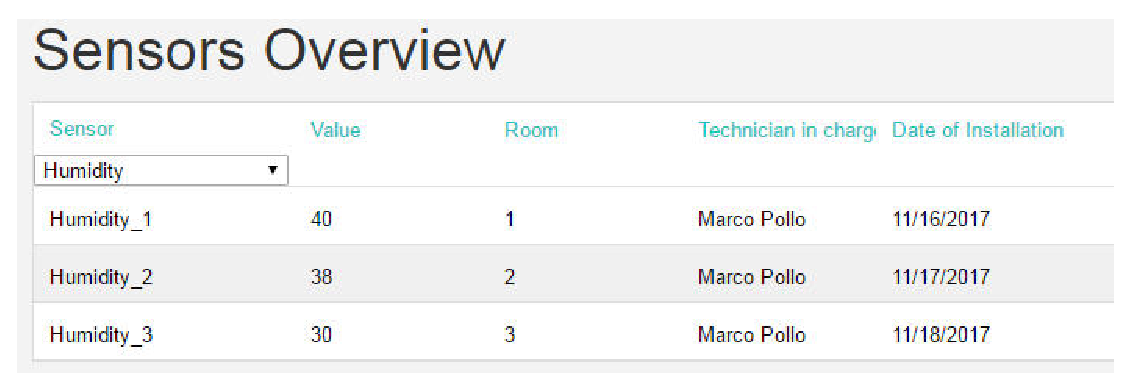
\includegraphics[width=1\textwidth]{images/HumiditySensor.eps}
\end{figure}
\end{enumerate}
\end{description}

\subsubsection{Example of humidity sensor sending digital signal}
\textbf{Humidity sensor 1} sends 40 as digital signal. \textbf{System} updates
the sensor table value from room 1 and humidity sensor1.
\hfill
\vspace{0.5cm}
\hrule


\subsection{Temperature sensor push information}

\hrule
\hfill
\vspace{0.5cm}
\label{operation:Temperature sensor push information}

The Temperature Sensor pushes the information to the sensor table.
\begin{description}
\item \textbf{Parameters:} 
\item \textbf{Precondition:} The system is bootedup with the respected
configurations.
\item \textbf{Post-condition:} Updated sensor value in sensor table.

\item \textbf{Triggering:}
\begin{enumerate}
\item \textbf{Temperature sensor} sends digital signal to the system.
\item System updates the value of the given temperature sensor in the sensor
table.
\item \begin{figure}[H]
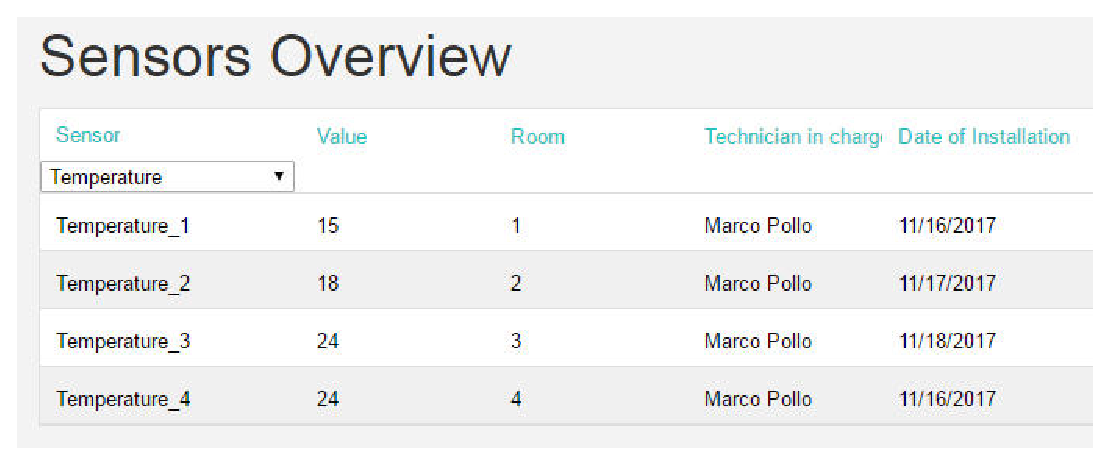
\includegraphics[width=1\textwidth]{images/TemperatureSensor.eps}
\end{figure}
\end{enumerate}
\end{description}

\subsubsection{Example of humidity sensor sending digital signal}
\textbf{Temperature sensor 1} sends 24 as digital signal. \textbf{System}
updates the sensor table value from room 1 and Temperature sensor1 by modifing
the value to 24.
\hfill
\vspace{0.5cm}
\hrule

\break

\subsection{Light sensor push information}

\hrule
\hfill
\vspace{0.5cm}
\label{operation:Light sensor push information}

The  Light Sensor pushes the information to the sensor table.
\begin{description}
\item \textbf{Parameters:} 
\item \textbf{Precondition:} The system is bootedup with the respected
configurations.
\item \textbf{Post-condition:} Updated Light value in sensor table of the given
Light sensor.

\item \textbf{Triggering:}
\begin{enumerate}
\item \textbf{Light sensor} sends digital signal to the system.
\item System updates the value of the given sensor in the sensor table.
\item \begin{figure}[H]
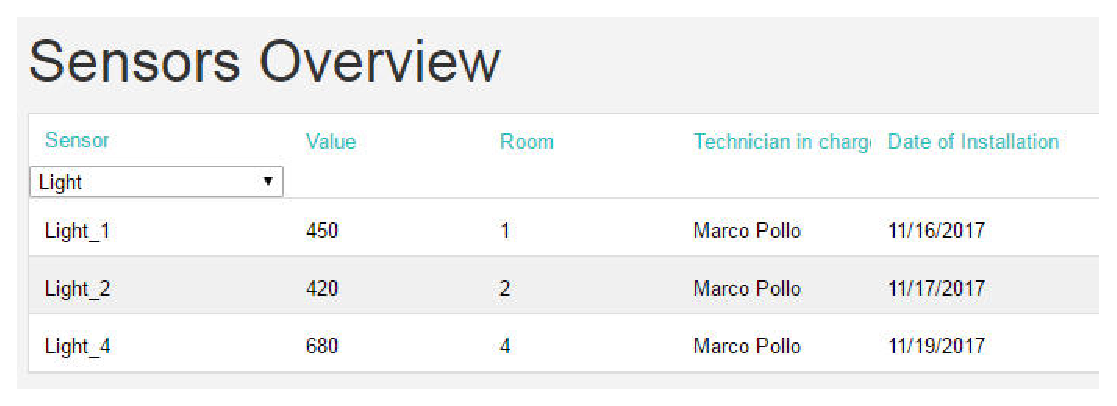
\includegraphics[width=1\textwidth]{images/LightSensor.eps}
\end{figure}
\end{enumerate}
\end{description}

\subsubsection{Example of humidity sensor sending digital signal}
\textbf{Light sensor 1} sends 550 nm as digital signal. \textbf{System}
updates the sensor table value from room 1 and updates the light value to 550nm.
\hfill
\vspace{0.5cm}
\hrule


\subsection{Motion sensor push information}

\hrule
\hfill
\vspace{0.5cm}
\label{operation:Motion sensor push information}

The Motion Sensor pushes the information to the sensor table.
\begin{description}
\item \textbf{Parameters:} \
\item \textbf{Precondition:} The system is bootedup with the respected
configurations.
\item \textbf{Post-condition:} The system sends alert to the manager.

\item \textbf{Triggering:}
\begin{enumerate}
\item \textbf{Motion sensor} sends digital signal to the system if any movement
is detected.
\item System displays an alert to the manager that there might be an intrusion.
\end{enumerate}
\end{description}

\subsubsection{Example of Motion sensor sending digital signal}
\textbf{Motion sensor 1} sends a digital signal to the system. The system alerts
the manager of an intrusion.
\hfill
\vspace{0.5cm}
\hrule

\break



\subsection{Turn on Heater}

\hrule
\hfill
\vspace{0.5cm}
\label{operation:Turn on heater}

In case the Temeprature sensor sends an a value less then 15 degrees the heater
is switched on.
\begin{description}
\item \textbf{Parameters:} temperatureOfSensor
\item \textbf{Precondition:} The system is bootedup with the respected
configurations and digital signals comming from the Temperature sensor which is
less then 15 degrees.
\item \textbf{Post-condition:} Heater in a given room is on until the
Temperature sensor sends value heigher than 19.

\item \textbf{Triggering:}
\begin{enumerate}
\item \textbf{Temperature sensor} sends digital signal of 14 to the system.
\item System enables the heater for the given room.
\item \item \begin{figure}[H]

\includegraphics[width=1\textwidth]{images/TurnOnHeater.eps}
\end{figure}
\end{enumerate}
\end{description}

\subsubsection{Example of humidity sensor sending digital signal}
\textbf{Temperature sensor 1} sends 14 as digital signal. \textbf{System}
enables the heater to heat the room1 until the temperature sensor sends a value
heigher than 18.
\hfill
\vspace{0.5cm}
\hrule


\subsection{Turn on LED}

\hrule
\hfill
\vspace{0.5cm}
\label{operation:Turn on LED}

Incase the light sensor pushes a value less than 400 the LEDs qre turned on.
\begin{description}
\item \textbf{Parameters:} lightValue,timeTicker
\item \textbf{Precondition:} The system is bootedup with the respected
configurations and digital signals comming from the Lightsensor has to be less
than 400 nm and the ticker has to be 0.
\item \textbf{Post-condition:} The LEDS for the given room are turned on until
the outside Lightsensor gives a value more than 400.

\item \textbf{Triggering:}
\begin{enumerate}
\item \textbf{Light sensor} sends digital signal of less than 400 nm to the
system.
\item System enables the LEDs for the given room if the TimeTicker is 0.
\item \begin{figure}[H]

\includegraphics[width=1\textwidth]{images/LEDSON.eps}
\end{figure}
\end{enumerate}
\end{description}

\subsubsection{Example of humidity sensor sending digital signal}
\textbf{Light sensor 1} sends 399 as digital signal. \textbf{System}
evaluates if the timeTicker is 0 if it is it turns the LEDs on.
\hfill
\vspace{0.5cm}
\hrule

\subsection{Open Windows}

\hrule
\hfill
\vspace{0.5cm}
\label{operation:Open Windows}

Incase the temperature sensor inside has a value higher than the value allowed.
\begin{description}
\item \textbf{Parameters:} Temperature,room,TemperatureSHouldBE
\item \textbf{Precondition:} The system is bootedup with the respected
configurations and digital signals comming from the Temperature sensor has to be
more than a given value.
\item \textbf{Post-condition:} The Windows for that given room are opend.

\item \textbf{Triggering:}
\begin{enumerate}
\item \textbf{Temperature sensor} sends digital signal of more than a given
value degrees to the system.
\item System opens the windows unitl the temperature decreeces to the requested
temperature.
\end{enumerate}
\end{description}

\subsubsection{Example of humidity sensor sending digital signal}
\textbf{Temperature sensor 1} sends 45 (degree) as digital signal.
\textbf{System} checks if the temperature is acceding the temperature should be
than the windows are opening.
\begin{figure}[H]
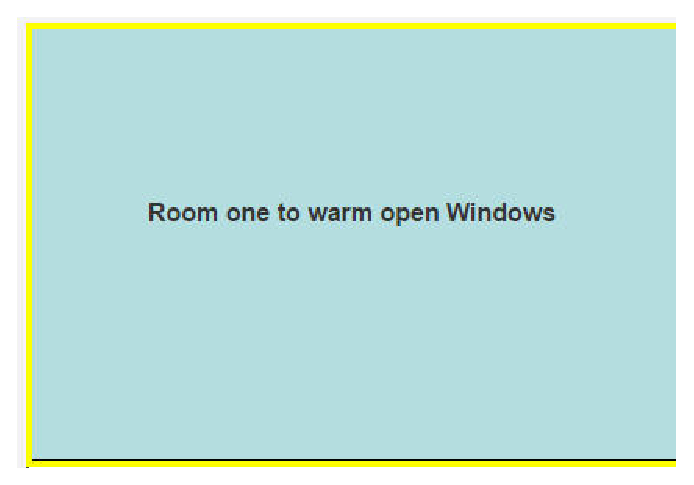
\includegraphics[width=1\textwidth]{images/OpenWindows.eps}
\end{figure}
\hfill
\vspace{0.5cm}
\hrule









\subsection{Turn on watering}

\hrule
\hfill
\vspace{0.5cm}
\label{operation:Turn on watering}

Incase the humidty sensor gives a value below the requested value watering is
turned on.
\begin{description}
\item \textbf{Parameters:} humidityLevel,Room
\item \textbf{Precondition:} The system is bootedup with the respected
configurations and digital signals comming from the humidty sensor has to be
less than a given level.
\item \textbf{Post-condition:} The watering is turned on for the given room.

\item \textbf{Triggering:}
\begin{enumerate}
\item \textbf{Humidty sensor} sends digital signal of less than the accepted
amount to the system.
\item System enables the watering for a given room until the humidty level is
as the room humidtyi accepts it.
\end{enumerate}
\end{description}

\subsubsection{Example of Enabling wateringl}
\textbf{Humidity sensor 1} sends a value of 10 since the humidity sensor is in
room1.
\textbf{System} enables the watering for the room1 until the humidity level is
40 so that the plants have enough water.
\begin{figure}[H]
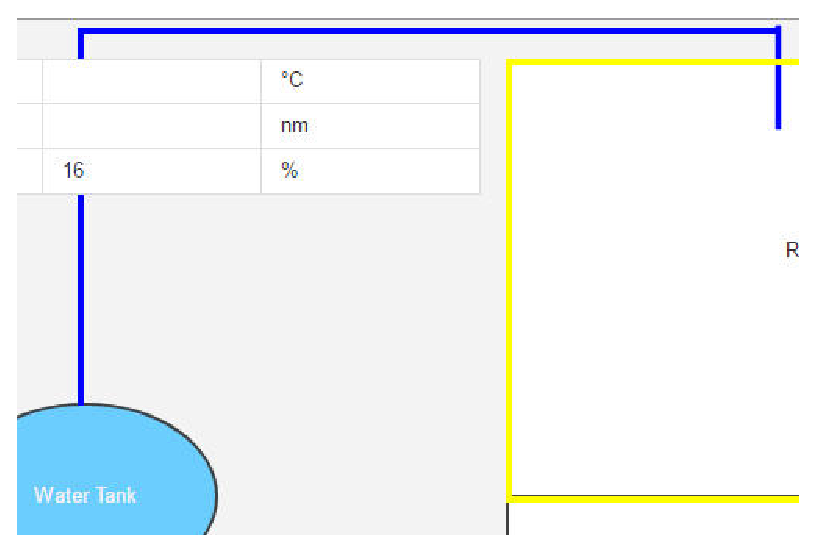
\includegraphics[width=1\textwidth]{images/WateringOn.eps}
\end{figure}
\hfill
\vspace{0.5cm}
\hrule
